\documentclass[11pt,a4paper]{article}
    \usepackage[margin=2.5cm]{geometry}
    \usepackage{enumitem}
    \usepackage{hyperref}
    \usepackage{tikz}
    \usetikzlibrary{arrows.meta,positioning,shapes.geometric}
    \title{Chemoinformatics Tools}
\author{Jordi Vill\`a-Freixa \texttt{<jordi.villa@uvic.cat>}}
    \date{\today}

    \tikzset{
      methodbox/.style={
        rounded corners=6pt,
        draw=blue!50!black,
        line width=0.9pt,
        fill=blue!6,
        minimum width=13cm,
        text width=11.8cm,
        align=left,
        inner sep=8pt
      }
    }

    \begin{document}
    \maketitle

    \section*{Scope}
    This folder provides notebook-driven chemoinformatics examples built around RDKit and public chemical databases such as ChEMBL.

    \section*{Material in this folder}
    \begin{itemize}[leftmargin=*]
\item \texttt{IdentifyFG.ipynb}
\item \texttt{chembl.ipynb}
\item \texttt{smilesRDKIT.ipynb}
\item \texttt{ifgutil.py}
    \end{itemize}

    \section*{Method summary}
    \begin{itemize}[leftmargin=*]
\item \textbf{SMILES parsing and descriptor handling}. The RDKit notebooks convert textual molecular representations into molecular graphs for downstream analysis.
\item \textbf{Functional-group identification}. The helper module annotates atoms with functional-group labels and prepares one-hot encodings of those annotations.
\item \textbf{Database retrieval from ChEMBL}. The ChEMBL notebook illustrates how to query compound information and turn it into analyzable tables.
\item \textbf{Small-molecule educational workflows}. The examples emphasize interpretable cheminformatics manipulations rather than high-throughput screening pipelines.
    \end{itemize}

    \section*{Method scheme}
    Figure~\ref{fig:summary} is drawn directly in LaTeX with TikZ. It is a compact conceptual map of the main workflows discussed in this folder.

    \begin{figure}[ht]
    \centering
    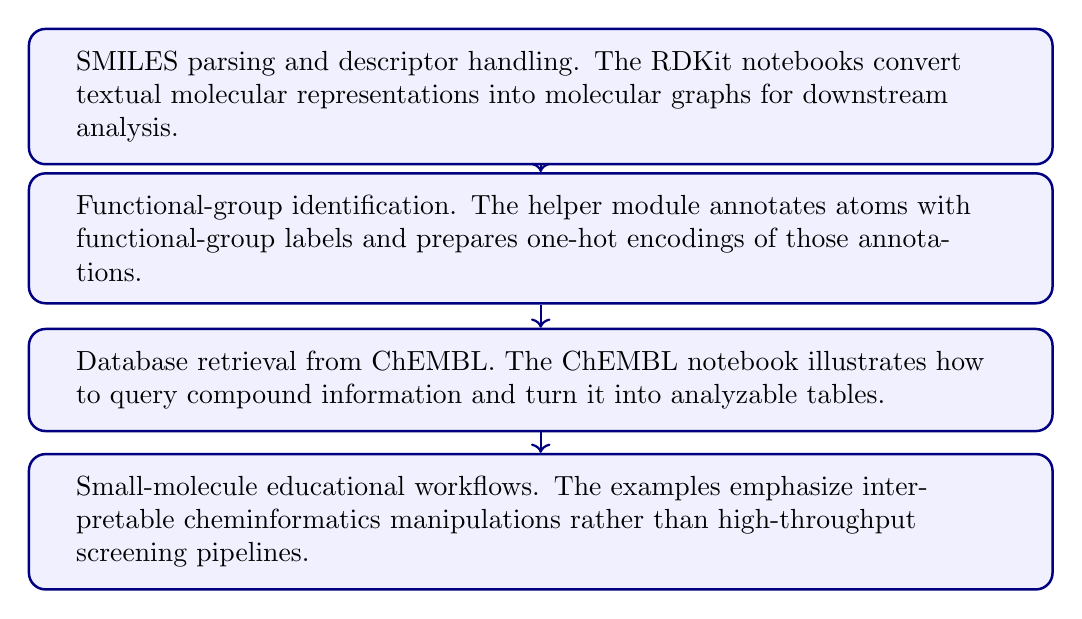
\begin{tikzpicture}[x=1cm,y=1cm]
    \node[methodbox] (m0) at (0,0.0) {SMILES parsing and descriptor handling. The RDKit notebooks convert textual molecular representations into molecular graphs for downstream analysis.};
    \node[methodbox] (m1) at (0,-1.8) {Functional-group identification. The helper module annotates atoms with functional-group labels and prepares one-hot encodings of those annotations.};
    \node[methodbox] (m2) at (0,-3.6) {Database retrieval from ChEMBL. The ChEMBL notebook illustrates how to query compound information and turn it into analyzable tables.};
    \node[methodbox] (m3) at (0,-5.4) {Small-molecule educational workflows. The examples emphasize interpretable cheminformatics manipulations rather than high-throughput screening pipelines.};
    \draw[->, thick, color=blue!50!black] (m0.south) -- (m1.north);
    \draw[->, thick, color=blue!50!black] (m1.south) -- (m2.north);
    \draw[->, thick, color=blue!50!black] (m2.south) -- (m3.north);
    \end{tikzpicture}
    \caption{Conceptual scheme for the methods in the chemoinformaticsTools folder.}
    \label{fig:summary}
    \end{figure}

    
\section*{Disclaimer}
These documents were generated with the assistance of ChatGPT 5.4. The material has been reviewed by the author before inclusion in this repository, but it is not free from possible errors.

\end{document}